\apendice{Especificación de diseño}

\section{Introducción}
Una vez realizado el estudio y especificación de los requisitos de la aplicación web, se debe realizar el diseño de la misma.\\
En este anexo se pretende aportar información sobre el diseño de los datos que utiliza la aplicación junto al diseño procedimental y arquitectónico del proyecto.

\section{Diseño de datos}
Gracias a la especificación de requisitos y casos de uso, se puede obtener una visión global de la aplicación que permite deducir las entidades, acompañadas de sus datos, necesarias para poder cumplir con lo requerido.\\
En primer lugar, podemos obtener la visión global de las entidades relacionadas mediante el diagrama general de Entidad-Relación de la figura~\ref{DiagramaGeneralE-R}.\\
El diagrama obtenido tiene un gran tamaño y, para mejorar la visualización y comprensión del mismo, se ha decidido dividir en vistas donde se incluyan los datos de cada una de las entidades.\\
La primera vista hace referencia al apartado de mantenimiento académico y se puede ver en la figura~\ref{er_cu1}, la segunda al mantenimiento de profesorado~\ref{er_cu2} y la última a la asignación docente~\ref{er_cu3}.

\begin{landscape}
	\begin{figure}[h]
		\caption{Diagrama general entidad-relación}
		\centering
		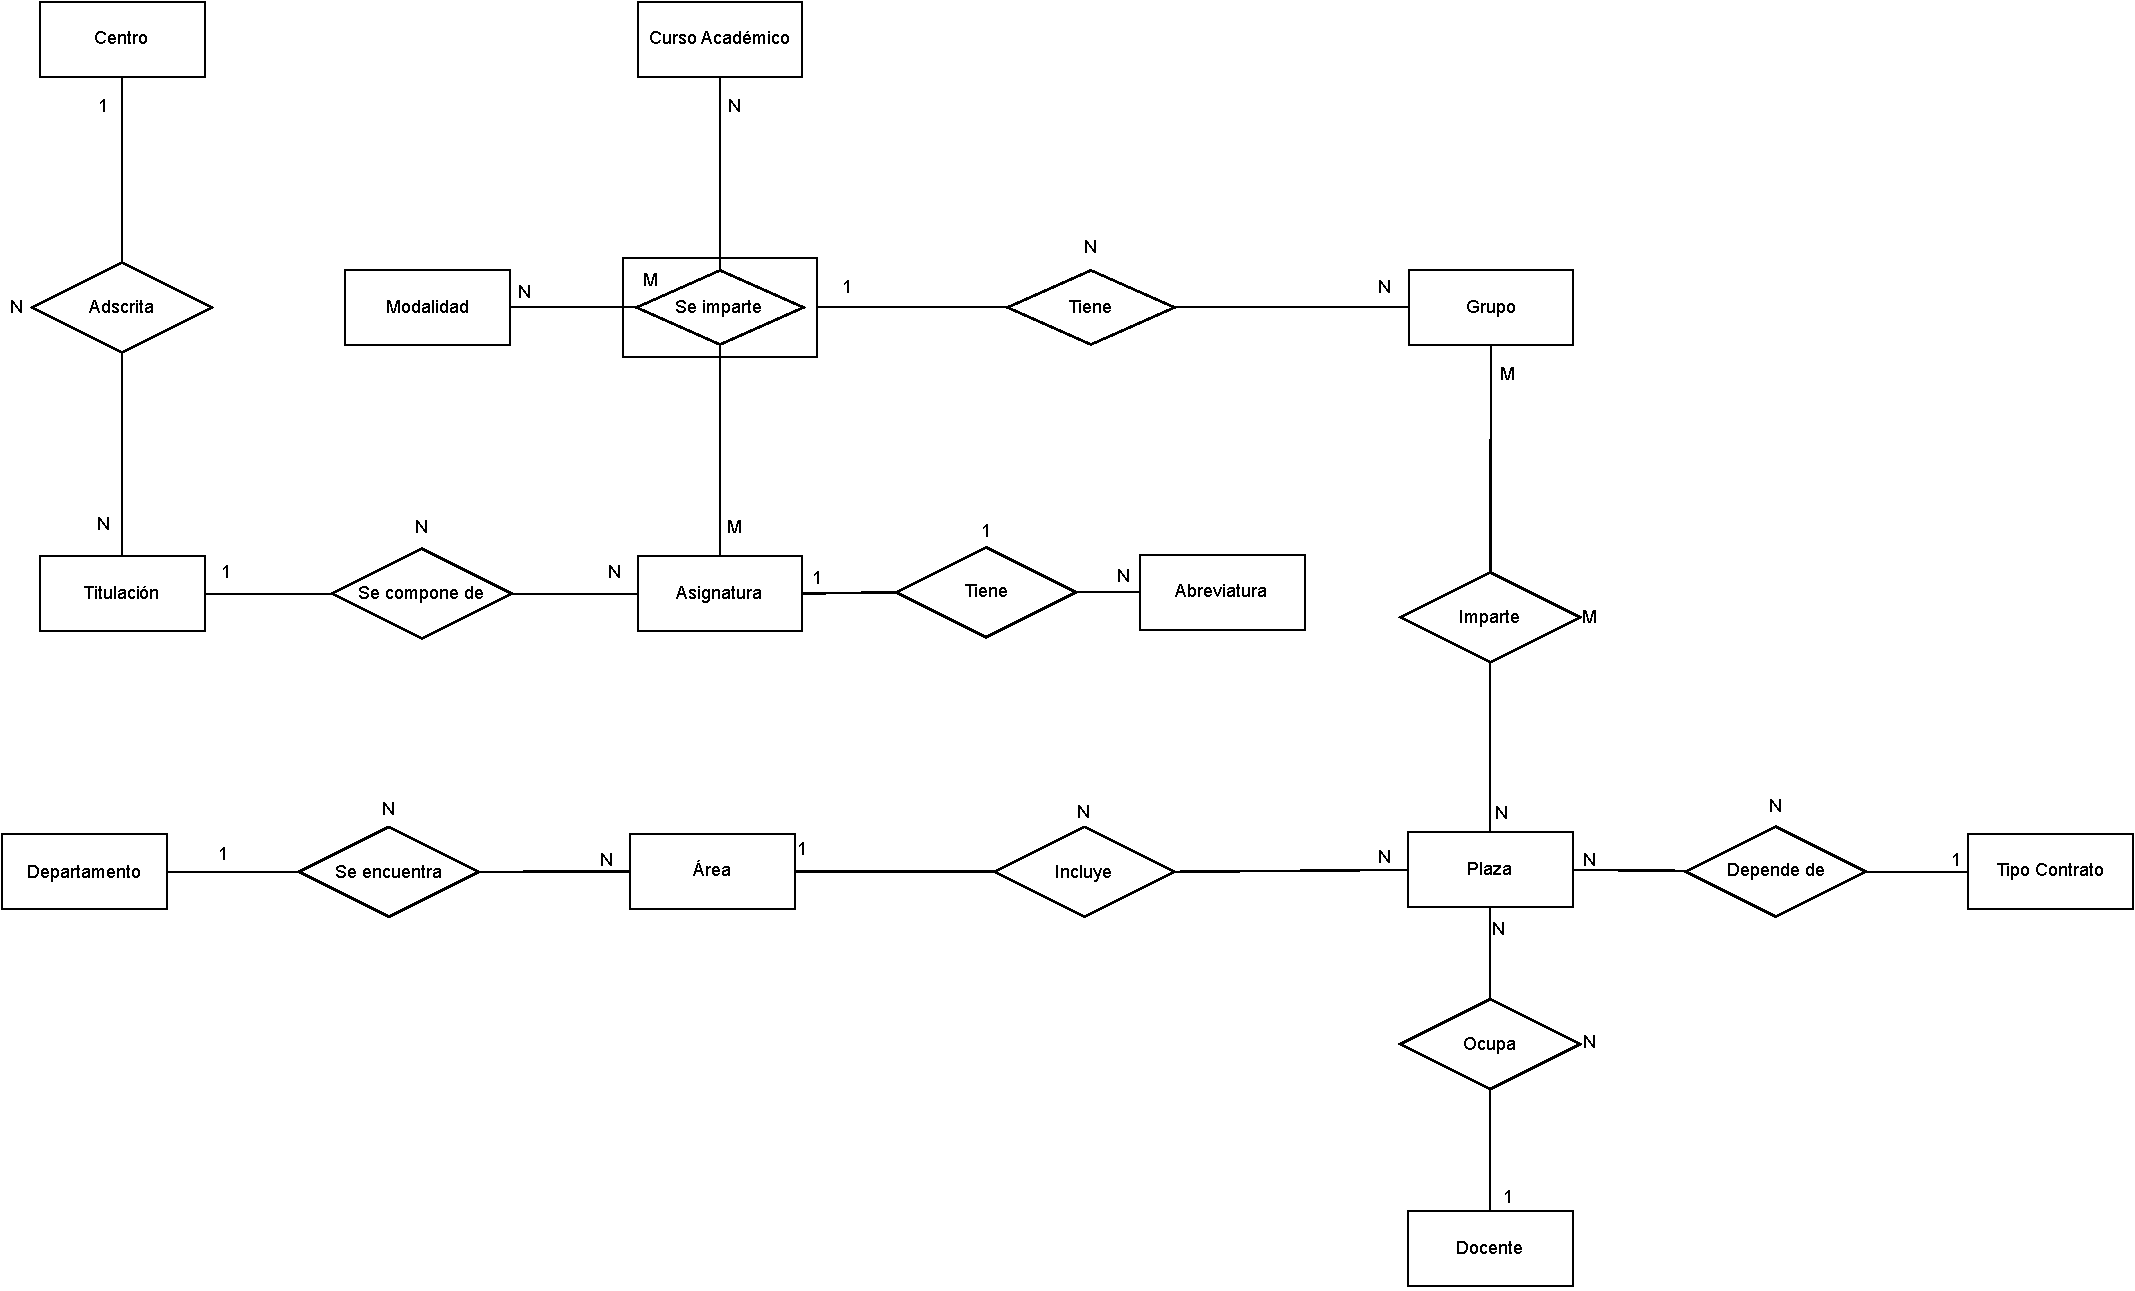
\includegraphics[scale=0.65]{../img/Anexos/Diagrama E-R.pdf}
		\label{DiagramaGeneralE-R}
	\end{figure}
\end{landscape}

Del diagrama entidad-relación se puede obtener el diagrama relacional de la figura~\ref{DiagramaRelacional} en el que se pueden ver la tablas que contendrá la base de datos de la aplicación web.

En este diagrama se pueden ver las tablas de la base de datos juntos los distintos campos que tendrá cada una.
Como se puede ver en la figura~\ref{DiagramaRelacional}, las tablas centro, titulación y asignatura tienen un campo llamado código. 
Este código campo podría haber sido utilizado como clave primaria, pero al ser un campo que introduce el usuario, se decidió mantener una clave primaria auto-incremental con la que se hacen las relaciones de las tablas, y además, añadir ese campo para que se puedan hacer búsquedas o filtrar por el mismo sin que su uso pueda afectar a la consistencia del sistema.

Otro aspecto relevante es que en las relaciones que dan lugar a la creación de una tabla intermedia se siguió el mismo patrón que antes. 
Aunque la teoría diga que las claves de las tablas que se relacionan pasan a ser claves primarias de la nueva tabla que se genera, se decidió tener una única clave primaria auto-incremental y tener las claves de las tablas relacionadas como claves foráneas.
De esta manera, las búsquedas en la base de datos estarán más optimizadas al buscar como clave primaria un único campo y no la composición de varios.
Además, se evita cualquier tipo de error de clave primaria al ser la propia base de datos la que asigna esta y no el código creado.

\begin{landscape}
	\begin{figure}[h]
		\caption[DiagramaRelacional]{Diagrama relacional}
		\centering
		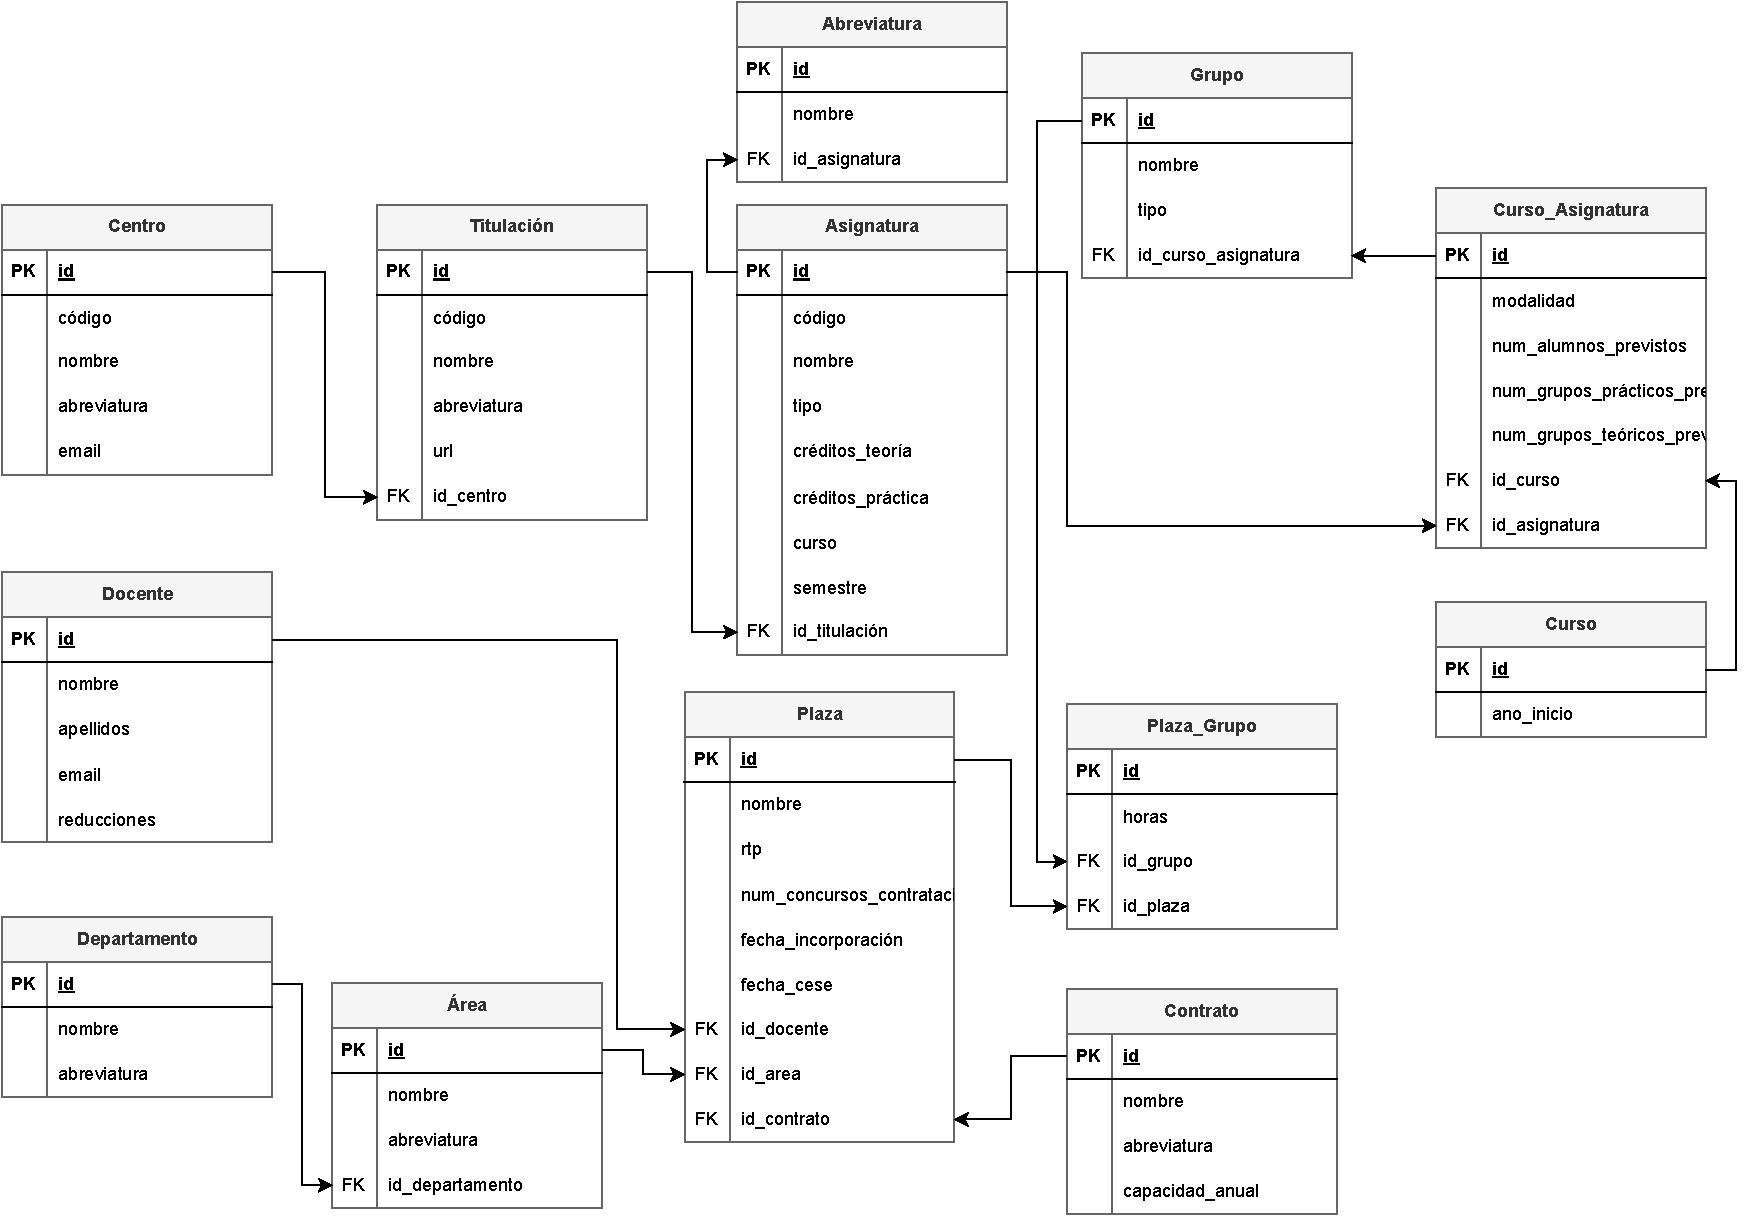
\includegraphics[scale=0.7]{../img/Anexos/Diagrama relacional.pdf}
		\label{DiagramaRelacional}
	\end{figure}
\end{landscape}

\subsection{Diccionario de datos}
A continuación se va a especificar, para cada tabla de la base de datos, el diccionario de datos correspondiente.
De esta forma se pretende facilitar la comprensión de los datos almacenados en la base de datos.
\subsubsection{Tabla Centro}
La tabla \texttt{centro} almacena los diferentes centros de la universidad. 
Se puede ver su información en la tabla~\ref{tab:diccionario_centro}.
\begin{table}
\centering
  \begin{tabular}{l p{.2\textwidth} p{.5\textwidth}}
    \toprule
    \textbf{Campo} & \textbf{Tipo} & \textbf{Descripción}\\
    \midrule
    \textbf{\underline{id}} & Entero \underline{PK} & Identificador. Clave primaria creada de forma autoincremental. \\ \addlinespace
    codigo & Entero & Código interno del centro de la universidad. Sólo tiene carácter informativo. \\ \addlinespace 
    abreviatura & Texto & Abreviatura del centro. \\ \addlinespace
    email & Texto & Email administrativo del centro. \\
    \bottomrule
  \end{tabular}
  \caption{Diccionario de datos. Tabla Centro}
  \label{tab:diccionario_centro}
\end{table}

\subsubsection{Tabla Titulación}
La tabla \texttt{titulación} almacena las titulaciones que son creadas y que pertenecen a un centro.
Se puede ver su información en la tabla~\ref{tab:diccionario_titulacion}.
\begin{table}
  \centering 
  \begin{tabular}{l p{.2\textwidth} p{.5\textwidth}}
    \toprule
    \textbf{Campo} & \textbf{Tipo} & \textbf{Descripción}\\
    \midrule
    \textbf{\underline{id}} & Entero \underline{PK} & Identificador de la titulación. Clave primaria creada de forma autoincremental. \\ \addlinespace
    codigo & Entero & Código interno de la titulación. \\ \addlinespace
    nombre & Texto & Nombre de la titulación. \\ \addlinespace
    abreviatura & Texto & Abreviatura de la titulación. \\ \addlinespace
    url & Texto & Dirección web de la titulación. \\ \addlinespace
    id\_centro & Entero FK(Centro) & Identificador del centro asociado a la titulación. \\
    \bottomrule
  \end{tabular}
  \caption{Diccionario de datos. Tabla Titulación}
  \label{tab:diccionario_titulacion}
\end{table}

\subsubsection{Tabla Asignatura}
La tabla \texttt{asignatura} almacena información sobre las asignaturas, cada asignatura pertenece a una titulación. Se puede ver su información en la Tabla~\ref{tab:diccionario_asignatura}.

\begin{table}
  \centering 
  \begin{tabular}{l p{.2\textwidth} p{.5\textwidth}}
    \toprule
    \textbf{Campo} & \textbf{Tipo} & \textbf{Descripción}\\
    \midrule
    \textbf{\underline{id}} & Entero \underline{PK} & Identificador de la asignatura. Clave primaria creada de forma autoincremental. \\ \addlinespace
    codigo & Entero & Código interno de la asignatura. \\ \addlinespace
    nombre & Texto & Nombre de la asignatura. \\ \addlinespace
    tipo & Texto & Tipo de la asignatura. \\ \addlinespace
    creditos\_teoria & Entero & Créditos de teoría de la asignatura. \\ \addlinespace
    creditos\_practica & Entero & Créditos de práctica de la asignatura. \\ \addlinespace
    curso & Texto & Curso al que pertenece la asignatura. \\ \addlinespace
    semestre & Texto & Semestre en el que se imparte la asignatura. \\ \addlinespace
    id\_titulacion & Entero FK(Titulación) & Identificador de la titulación a la que pertenece la asignatura. \\
    \bottomrule
  \end{tabular}
  \caption{Diccionario de datos. Tabla Asignatura}
  \label{tab:diccionario_asignatura}
\end{table}

\subsubsection{Tabla Abreviatura}
La tabla \texttt{abreviatura} almacena las abreviaturas de las asignaturas. 
De esta forma se permite que una asignatura pueda tener varias abreviaturas.
Se puede ver su información en la tabla~\ref{tab:diccionario_abreviatura}.

\begin{table}
  \centering 
  \begin{tabular}{l p{.2\textwidth} p{.5\textwidth}}
    \toprule
    \textbf{Campo} & \textbf{Tipo} & \textbf{Descripción}\\
    \midrule
    \textbf{\underline{id}} & Entero \underline{PK} & Identificador de la abreviatura. Clave primaria creada de forma autoincremental. \\ \addlinespace
    abreviatura & Texto & Abreviatura de la asignatura. \\ \addlinespace
    id\_asignatura & Entero FK(Asignatura) & Identificador de la asignatura asociada a la abreviatura. \\
    \bottomrule
  \end{tabular}
  \caption{Diccionario de datos. Tabla Abreviatura}
  \label{tab:diccionario_abreviatura}
\end{table}


\subsubsection{Tabla Curso}
La tabla \texttt{curso} almacena información sobre los cursos. Se puede ver su información en la Tabla~\ref{tab:diccionario_curso}.

\begin{table}
  \centering 
  \begin{tabular}{l p{.2\textwidth} p{.5\textwidth}}
    \toprule
    \textbf{Campo} & \textbf{Tipo} & \textbf{Descripción}\\
    \midrule
    \textbf{\underline{id}} & Entero \underline{PK} & Identificador del curso. Clave primaria creada de forma autoincremental. \\ \addlinespace
    ano\_inicio & Texto & Año de inicio del curso. \\ \addlinespace
    \bottomrule
  \end{tabular}
  \caption{Diccionario de datos. Tabla Curso}
  \label{tab:diccionario_curso}
\end{table}

\subsubsection{Tabla Curso-Asignatura}
La tabla \texttt{curso\_asignatura} almacena la relación entre cursos y asignaturas. 
Se puede ver su información en la Tabla~\ref{tab:diccionario_curso_asignatura}.

\begin{table}
  \centering
  \begin{tabular}{l p{.2\textwidth} p{.25\textwidth}}
    \toprule
    \textbf{Campo} & \textbf{Tipo} & \textbf{Descripción}\\
    \midrule
    \textbf{\underline{id}} & Entero \underline{PK} & Identificador de la relación curso-asignatura. Clave primaria creada de forma autoincremental. \\ \addlinespace
    id\_asignatura & Entero FK(Asignatura) & Identificador de la asignatura relacionada. \\ \addlinespace
    id\_curso & Entero FK(Curso) & Identificador del curso relacionado. \\ \addlinespace
    modalidad & Texto & Modalidad de la relación curso-asignatura. \\ \addlinespace
    num\_alumnos\_previstos & Entero & Número de alumnos previstos para la relación curso-asignatura. \\ \addlinespace
    num\_grupos\_teoricos\_previstos & Entero & Número de grupos teóricos previstos para la relación curso-asignatura. \\ \addlinespace
    num\_grupos\_practicos\_previstos & Entero & Número de grupos prácticos previstos para la relación curso-asignatura. \\
    \bottomrule
  \end{tabular}
  \caption{Diccionario de datos. Tabla Curso-Asignatura}
  \label{tab:diccionario_curso_asignatura}
\end{table}

\subsubsection{Tabla Grupo}
La tabla \texttt{grupo} almacena información sobre los grupos de asignaturas. 
Se puede ver su información en la Tabla~\ref{tab:diccionario_grupo}.

\begin{table}
  \centering 
  \begin{tabular}{l p{.2\textwidth} p{.4\textwidth}}
    \toprule
    \textbf{Campo} & \textbf{Tipo} & \textbf{Descripción}\\
    \midrule
    \textbf{\underline{id}} & Entero \underline{PK} & Identificador del grupo. Clave primaria creada de forma autoincremental. \\ \addlinespace
    nombre & Texto & Nombre del grupo. \\ \addlinespace
    tipo & Texto & Tipo de grupo. \\ \addlinespace
    id\_curso\_asignatura & Entero FK(Curso-Asignatura) & Identificador de la relación curso-asignatura asociada al grupo. \\
    \bottomrule
  \end{tabular}
  \caption{Diccionario de datos. Tabla Grupo}
  \label{tab:diccionario_grupo}
\end{table}

\subsubsection{Tabla Docente}
La tabla \texttt{docente} almacena información sobre los docentes. Se puede ver su información en la Tabla~\ref{tab:diccionario_docente}.

\begin{table}
  \centering 
  \begin{tabular}{l p{.2\textwidth} p{.5\textwidth}}
    \toprule
    \textbf{Campo} & \textbf{Tipo} & \textbf{Descripción}\\
    \midrule
    \textbf{\underline{id}} & Entero \underline{PK} & Identificador del docente. Clave primaria generada de forma autoincremental. \\ \addlinespace
    nombre & Texto & Nombre del docente. \\ \addlinespace
    apellidos & Texto & Apellidos del docente. \\ \addlinespace
    email & Texto & Email del docente \\ \addlinespace
    reducciones & Entero & Número de horas de reducciones del docente. \\
    \bottomrule
  \end{tabular}
  \caption{Diccionario de datos. Tabla Docente}
  \label{tab:diccionario_docente}
\end{table}


\subsubsection{Tabla Departamento}
La tabla \texttt{departamento} almacena información sobre los departamentos de la universidad. 
Se puede ver su información en la Tabla~\ref{tab:diccionario_departamento}.

\begin{table}
  \centering 
  \begin{tabular}{l p{.2\textwidth} p{.5\textwidth}}
    \toprule
    \textbf{Campo} & \textbf{Tipo} & \textbf{Descripción}\\
    \midrule
    \textbf{\underline{id}} & Entero \underline{PK} & Identificador del departamento. Clave primaria generada de forma autoincremental. \\ \addlinespace
    nombre & Texto & Nombre del departamento. \\ \addlinespace
    abreviatura & Texto & Abreviatura del departamento. \\
    \bottomrule
  \end{tabular}
  \caption{Diccionario de datos. Tabla Departamento}
  \label{tab:diccionario_departamento}
\end{table}

\subsubsection{Tabla Área}
La tabla \texttt{área} almacena información sobre las áreas de un departamento. 
Se puede ver su información en la Tabla~\ref{tab:diccionario_area}.

\begin{table}
  \centering 
  \begin{tabular}{l p{.2\textwidth} p{.5\textwidth}}
    \toprule
    \textbf{Campo} & \textbf{Tipo} & \textbf{Descripción}\\
    \midrule
    \textbf{\underline{id}} & Entero \underline{PK} & Identificador del área. Clave primaria creada de forma autoincremental. \\ \addlinespace
    nombre & Texto & Nombre del área. \\ \addlinespace
    abreviatura & Texto & Abreviatura del área. \\ \addlinespace
    id\_departamento & Entero FK(Departamento) & Identificador del departamento al que pertenece el área. \\
    \bottomrule
  \end{tabular}
  \caption{Diccionario de datos. Tabla Área}
  \label{tab:diccionario_area}
\end{table}

\subsubsection{Tabla Contrato}
La tabla \texttt{contrato} almacena información sobre los tipos de contratos. Se puede ver su información en la Tabla~\ref{tab:diccionario_tipo_contrato}.

\begin{table}
  \centering 
  \begin{tabular}{l p{.2\textwidth} p{.5\textwidth}}
    \toprule
    \textbf{Campo} & \textbf{Tipo} & \textbf{Descripción}\\
    \midrule
    \textbf{\underline{id}} & Entero \underline{PK} & Identificador del tipo de contrato. Clave primaria generada de forma autoincremental. \\ \addlinespace
    nombre & Texto & Nombre del tipo de contrato. \\ \addlinespace
    abreviatura & Texto & Abreviatura del tipo de contrato. \\ \addlinespace
    capacidad\_anual & Entero & Capacidad anual en horas del tipo de contrato. \\
    \bottomrule
  \end{tabular}
  \caption{Diccionario de datos. Tabla Tipo Contrato}
  \label{tab:diccionario_tipo_contrato}
\end{table}

\subsubsection{Tabla Plaza}
La tabla \texttt{plaza} almacena información sobre las plazas de contratación. Se puede ver su información en la Tabla~\ref{tab:diccionario_plaza}.

\begin{table}
  \centering 
  \begin{tabular}{l p{.2\textwidth} p{.35\textwidth}}
    \toprule
    \textbf{Campo} & \textbf{Tipo} & \textbf{Descripción}\\
    \midrule
    \textbf{\underline{id}} & Entero \underline{PK} & Identificador de la plaza. Clave primaria generada de forma autoincremental \\ \addlinespace
    nombre & Texto & Nombre de la plaza \\ \addlinespace
    rpt & Texto & RPT de la plaza \\ \addlinespace
    num\_concursos\_contratacion & Entero & Número de concursos de contratación de la plaza \\ \addlinespace
    fecha\_incorporacion & Fecha & Fecha de incorporación a la plaza. \\ \addlinespace
    fecha\_cese & Fecha & Fecha de cese de la plaza. \\ \addlinespace
    id\_docente & Entero & Identificador del docente asignado a la plaza. \\ \addlinespace
    id\_area & Entero & Identificador del área asociada a la plaza. \\ \addlinespace
    id\_contrato & Entero & Identificador del tipo de contrato asociado a la plaza. \\
    \bottomrule
  \end{tabular}
  \caption{Diccionario de datos. Tabla Plaza}
  \label{tab:diccionario_plaza}
\end{table}

\subsubsection{Tabla Plaza-Grupo}
La tabla \texttt{plaza-grupo} almacena información sobre la asignación de horas de plazas a grupos. Se puede ver su información en la Tabla~\ref{tab:diccionario_plaza_grupo}.

\begin{table}
  \centering 
  \begin{tabular}{l p{.2\textwidth} p{.5\textwidth}}
    \toprule
    \textbf{Campo} & \textbf{Tipo} & \textbf{Descripción}\\
    \midrule
    \textbf{\underline{id}} & Entero \underline{PK} & Identificador de la asignación. Clave primaria generada de forma autoincremental. \\ \addlinespace
    horas & Entero & Horas de la plaza asignadas al grupo. \\ \addlinespace
    id\_grupo & Entero & Identificador del grupo. \\ \addlinespace
    id\_plaza & Entero & Identificador de la plaza. \\
    \bottomrule
  \end{tabular}
  \caption{Diccionario de datos. Tabla Plaza-Grupo}
  \label{tab:diccionario_plaza_grupo}
\end{table}


\section{Diseño procedimental}
El diseño procedimental es una fase fundamental en el desarrollo de proyectos informáticos, donde se establecen los pasos necesarios para realizar una actividad dentro de la aplicación.


\section{Diseño arquitectónico}


